\documentclass[12pt]{article}

\usepackage{dcolumn}
\usepackage{booktabs}
\usepackage{pdflscape}
\usepackage{graphicx}
\usepackage{placeins}
\usepackage{amsmath}
\usepackage{hyperref}
\usepackage[margin = 3cm]{geometry}
\linespread{1.5}
\usepackage{xepersian}
\settextfont{XB Zar}
\setdigitfont{XB Zar}

\begin{document}
\title{دامنه قیمت}
\author{سید مرتضی آقاجان‌زاده}
\maketitle

در بازار سهام تهران محدودیت‌های نوسان روزانه برای نماد‌ها به صورت متفاوت وجود‌ دارد. آیا این محدودیت روزانه سبب جلب توجه سرمایه‌گذاران به سهم شده و در بازده و حجم روزانه سهم تغییر ایجاد می‌کند و باعث جذب سرمایه گذاران حقیقی به سهم می‌شود؟

\section{مطالعات گذشته}
\subsection{\lr{Predictable behavior, profits, and attention}}
\label{s1.1}
این مقاله در صدد آن است در بازار سهام شانگهای در روزی که قیمت سهم به حد بالایی محدوده قیمتی برخورد می‌کند از خود بازده بالا، حجم بالا و پوشش خبری نشان می‌دهد. این اتفاق توجه سرمایه گذاران را جلب می‌کند. در بازار تعداد سهام بالایی وجود دارد و این اتفاق می‌تواند مجموعه تصمیم گیری سرمایه‌گذاران را محدود کند.این مقاله از داده‌های معاملات روزانه نماد در بازار، قیمت سهام و کلیه معاملات افراد در شهری خاص استفاده کرده‌است تا علاوه بر بررسی حجم معاملات بررسی کند که آیا سرمایه گذاران جدیدی با برخورد قیمت به حد نوسان به سهم جذب می‌شوند یا خیر.


جهت بررسی رفتار سرمایه‌گذاران حقیقی شاخص عدم توازن خالص خرید برای زمان $ t $ و $ t+1 $ را به صورت زیر تعریف می‌کند

\lr{\begin{equation}
\text{Imbalance}_{k,t}^{\text{Indiv}} = \frac{\text{Buys}_{k,t}^{\text{Indiv}} - \text{Sells}_{k,t}^{\text{Indiv}}}{\text{Buys}_{k,t}^{\text{Indiv}} + \text{Sells}_{k,t}^{\text{Indiv}}}
\label{e1}
\end{equation}}
و بیان می‌کند چنانچه برخورد قیمت به حد نوسان توجه سرمایه‌گذاران حقیقی را جذب می‌کند آنگاه این شاخص در دوره $ t+1 $ مثبت است.

از طرفی جهت بررسی حجم معاملات از ملاک‌های زیر استفاده می‌کند که طبعا مانند حال قبل، نیاز است این شاخص‌ها در روزی که قیمت به حد نوسان برخورد می‌کند مثبت باشند.

\lr{\begin{equation}
\text{Turn}_{k,t} = \frac{\text{Volume}(\text{RBM})_{k,t}}{\text{MarketCap(FreeFloat)}_{k,t}}
\label{e2}
\end{equation}}
\lr{\begin{equation}
\text{RelTurn}_{k,t} = \frac{\text{Turn}_{k,t}}{AVG(\text{Turn}_{k,t})}
\label{e3}
\end{equation}}

\begin{figure}[htbp]
\centering
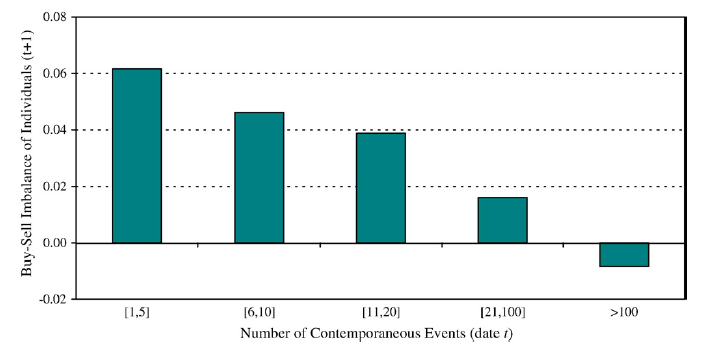
\includegraphics[width=\columnwidth]{g1.png}
\end{figure}
\FloatBarrier
\begin{figure}[htbp]
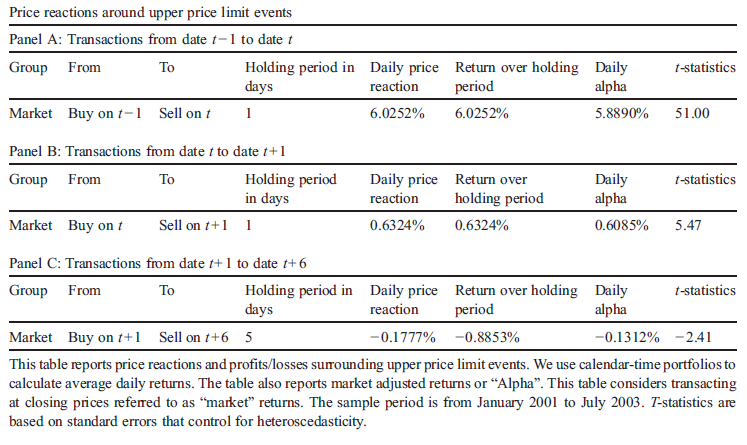
\includegraphics[width=\columnwidth]{Table4.png}
\caption{ نتایج  در مقاله بخش \ref {s1.1}}
\label{g2}
\end{figure}
\FloatBarrier
\subsection{\lr{Daily price limits and destructive market behavior}}
\label{s1.2}
در این مقاله در ابتدا بازده سهام در حوالی برخورد قیمت به دامنه نوسان بررسی شده‌است و پس از آن رفتار گونه‌های متفاوت سرمایه‌گذار مورد بررسی قرار گرفته است. در این مقاله از داده‌های در سطح حساب کاربری استفاده شده است.

این مقاله برای بررسی رفتار بازده سهام، از بازده‌های متفاوتی استفاده کرده‌است که در جدول 
\ref{t1} 
به صورت خلاصه بیان شده‌است. منظور از زمان $ t $ روزی است که اتفاق رخ می‌دهد. نتایج برآورد‌ها نیز در شکل
\ref{g1}
بیان شده‌است.
\begin{table}[htbp]
\centering
\begin{tabular}{|r|l|}
\hline
 توضیحات & متغیر\\
\hline

بازده قیمت پایانی نسبت به اولین قیمت در روز $ t $ & 
\lr{Close to open} \\

بازده اولین قیمت در روز $ t+1 $ نسبت به قیمت پایانی در روز $ t $ & 
\lr{Open to close} \\

بازده $ m $ روزه سهام & 
\lr{Day m } \\

بازده تجمعیی بین بازه $ m $ تا $ n $ روز بعد از دوره $ t $ & 
\lr{[m,n] } \\
\hline
\end{tabular}
\caption{خلاصه متغیر‌های وابسته تعریف شده در مقاله بخش \ref{s1.2}}
\label{t1}
\end{table}
کار دیگر مقاله بررسی رفتار سرمایه‌گذاران بزرگ در دوره t و t+1 می‌باشد که با توجه به دسترسی به داده‌های در سطح حساب کاربری این کار امکان پذیر بوده‌است.
نتایج در شکل 
\ref{g3}
نشان داده شده‌است.
\begin{figure}[htbp]
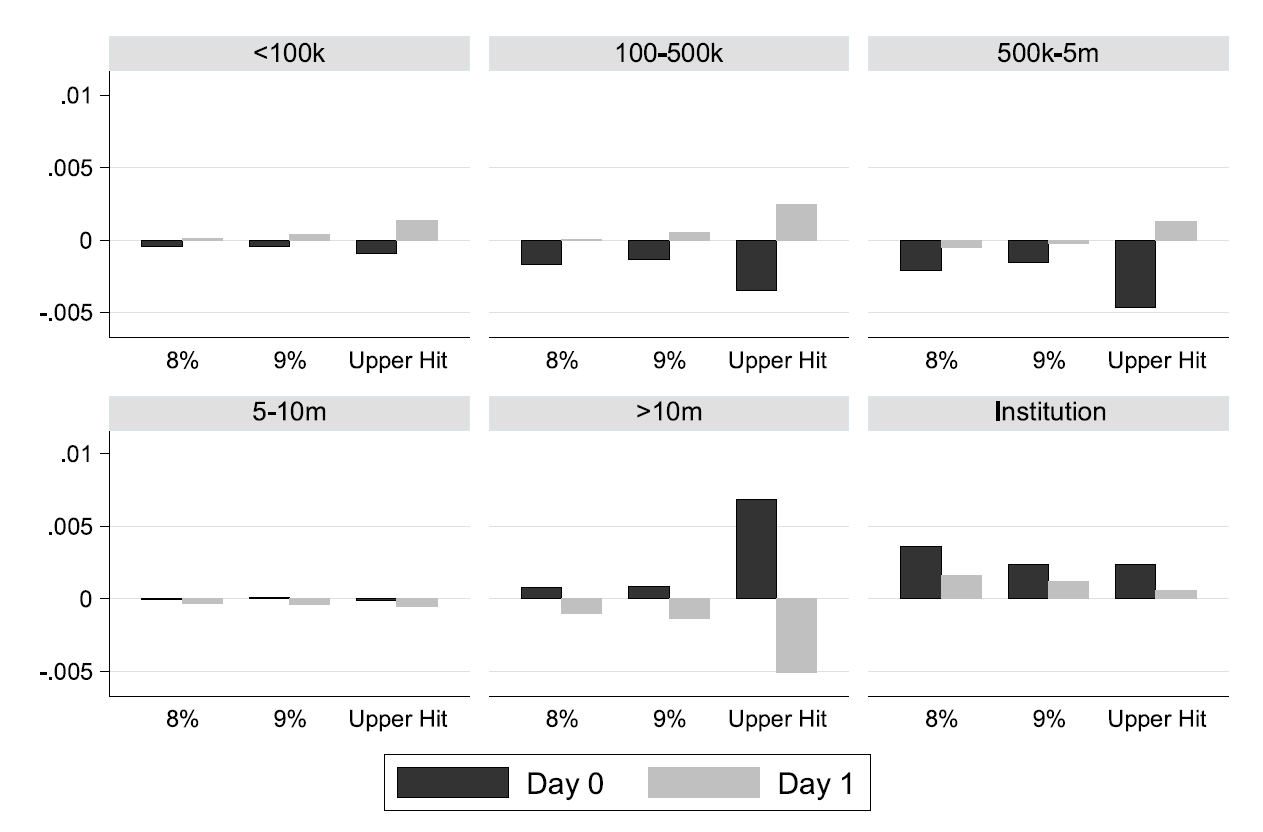
\includegraphics[width=1\columnwidth]{g2.png}
\caption{نتایج بررسی رفتار سرمایه‌گذاران عمده در مقاله بخش \ref {s1.2}}
\label{g3}
\end{figure}

\begin{landscape}
\begin{figure}[htbp]
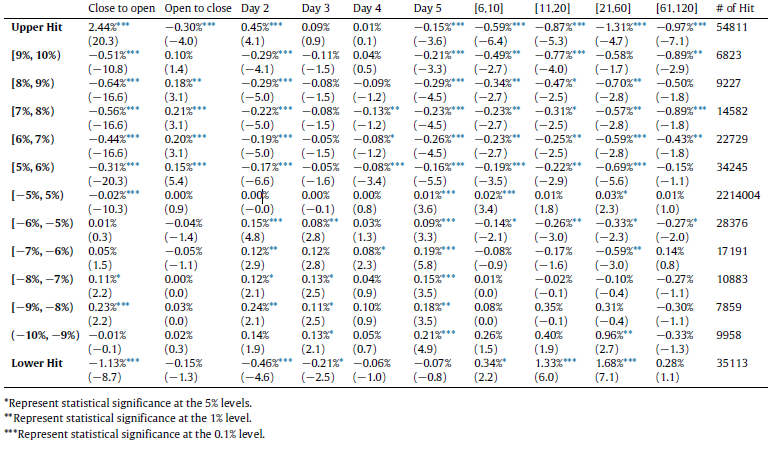
\includegraphics[width=1\columnwidth]{Table1.png}
\caption{خروجی نتایج رگرسیون در مقاله بخش \ref {s1.2}}
\label{g1}
\end{figure}
\end{landscape}
\FloatBarrier


\section{نتایج مقالات با استفاده از داده‌های ایران}
در بازار سهام ایران برخلاف بازار چین انوع مختلف دامنه نوسان وجود دارد. به همین علت به منظور کنترل حوادث متغیر‌های کنترل کننده دامنه نوسان به صورتی متفاوت تعریف شده‌اند. دو دسته متغیر‌های کنترلی تعریف می‌شود. در دسته اول 
($ \text{Upperhit} $ 
 و
 $ \text{Lowerhit} $)
برخورد حداکثر قیمت و حداقل قیمت معاملات به حد بالا و پایین نوسان بررسی می‌شود. در دسته دوم
($ \text{Upper} $ 
 و
 $ \text{Lower} $)
 قرار گرفتن حداکثر قیمت بالا‌تر از نصف حد بالای نوسان و حداقل قیمت کمتر از نصف حد پایین نوسان بررسی می‌شود. برای مثال چنانچه سهم دارای دامنه نوسان
  $ \pm 5 \% $
باشد برای متغیر 
$ \text{Upper} $
اگر درصد تغییرات حداکثر قیمت بیشتر مساوی 
$ 2.5 \%  $
باشد آنگاه متغیر فوق مقدار یک به خود می‌گیرد.
همچنین برای متغیر 
$ \text{Lower} $
نیز چنانچه درصد تغییرات حداقل قیمت کوچکتر مساوی 
$- 2.5 \%  $
 آنگاه متغیر فوق مقدار یک به خود می‌گیرد. لازم به ذکر است چنانچه قیمت به حد نوسان برخورد کند این متغیر‌ها مقدار صفر را می‌گیرند. از طرفی چنانچه با توجه به مثال حداکثر و حداقل قیمت معاملات در بازه 
 $ [-2.5\%,+2.5\%] $
 قرار گیرد متغییر $ Middle $ برابر یک قرار می‌گیرد.
 کنترل‌های دیگری همچون نوع دامنه نوسان، سهم از بازار نماد  و تغییر دامنه نوسان نیز مورد استفاده قرار گرفته‌است.


در ادامه در سه بخش مجزا بازده، حجم و خرید حقیقی سهام در روز‌های حادثه مورد بررسی قرار می‌گیرد.در هر بخش از داده‌های معاملات از سال 1396 تا انتهای 1398 استفاده شده‌است.


\subsection{بازده}
در این بخش از متغیر‌های وابسته تعریف شده در جدول 
\ref{t1}
استفاده شده‌است. ستون‌های 5 الی 8 جداول 
\ref{t2}-\ref{t4}
بازده تجمیعی میان روز‌های نوشته شده را نمایندگی می‌کنند. جدول 
\ref{t2}
و
\ref{t3}
رگرسیون ساده با دسته‌بندی به ترتیب در سطح زمان ($ t $) و در سطح نماد ($ id $) جهت محاسبه واریانس می‌باشد. جدول 
 \ref{t4}
 محاسبات همین معادلات به وسیله اثر ثابت در سطح نماد ($ id $) می‌باشد.



\newgeometry{top=15mm, bottom=25mm,left = 15mm,right = 15mm}

\begin{LTR}
\begin{landscape}
\begin{table}[htbp]
\centering
\lr{
\def\sym#1{\ifmmode^{#1}\else\(^{#1}\)\fi}
\begin{tabular}{l*{8}{c}}
\hline\hline
            &\multicolumn{1}{c}{(1)}&\multicolumn{1}{c}{(2)}&\multicolumn{1}{c}{(3)}&\multicolumn{1}{c}{(4)}&\multicolumn{1}{c}{(5)}&\multicolumn{1}{c}{(6)}&\multicolumn{1}{c}{(7)}&\multicolumn{1}{c}{(8)}\\
            &\multicolumn{1}{c}{closetoopen}&\multicolumn{1}{c}{opentoclose}&\multicolumn{1}{c}{ret\_1}&\multicolumn{1}{c}{ret\_2}&\multicolumn{1}{c}{ret\_2to5}&\multicolumn{1}{c}{ret\_5to50}&\multicolumn{1}{c}{ret\_50to100}&\multicolumn{1}{c}{ret\_100to300}\\
\hline
upperhit    &       3.487\sym{***}&      -1.139\sym{***}&       4.823\sym{***}&       7.806\sym{***}&       5.625\sym{***}&       11.02         &      -53.13\sym{**} &      1806.9         \\
            &     (15.39)         &    (-20.94)         &      (6.02)         &      (8.71)         &      (8.89)         &      (1.51)         &     (-2.60)         &      (1.31)         \\
[1em]
upper       &       1.595\sym{***}&      -0.820\sym{***}&       2.068\sym{***}&       3.142\sym{***}&       2.145\sym{***}&      -2.541         &      -49.55\sym{**} &     -1503.6         \\
            &      (8.03)         &    (-17.73)         &      (5.23)         &      (7.07)         &      (5.72)         &     (-0.40)         &     (-2.97)         &     (-1.34)         \\
[1em]
middle      &      -1.327\sym{***}&      -0.341\sym{***}&       0.962\sym{*}  &       2.120\sym{***}&       2.196\sym{***}&       49.85\sym{*}  &       229.5\sym{***}&       244.0         \\
            &     (-5.07)         &     (-6.71)         &      (2.10)         &      (4.06)         &      (5.77)         &      (2.38)         &      (4.23)         &      (0.19)         \\
[1em]
lower       &      -1.115\sym{***}&     -0.0994\sym{**} &      -0.659\sym{*}  &       0.625         &       4.211\sym{***}&       18.94\sym{***}&       56.53\sym{***}&       151.2         \\
            &     (-6.65)         &     (-2.63)         &     (-2.58)         &      (1.74)         &      (8.24)         &      (3.48)         &      (3.77)         &      (0.14)         \\
[1em]
lowerhit    &      -2.924\sym{***}&       0.488\sym{***}&      -3.181\sym{***}&      -3.064\sym{***}&       3.478\sym{***}&       31.58\sym{***}&       14.41         &      1911.6         \\
            &    (-10.72)         &      (5.67)         &     (-4.68)         &     (-4.03)         &      (6.99)         &      (7.88)         &      (1.10)         &      (1.42)         \\
[1em]
limitchange &       7.524\sym{***}&     -0.0248         &       11.07         &       16.15         &       0.797         &      -244.1\sym{*}  &     -1088.1\sym{***}&     16708.8\sym{***}\\
            &      (9.33)         &     (-0.37)         &      (1.38)         &      (1.90)         &      (0.80)         &     (-2.23)         &     (-4.15)         &      (3.81)         \\
\hline
\(N\)       &      119863         &      114831         &      119863         &      119598         &      118628         &      106075         &      101503         &       70705         \\
\hline\hline
\multicolumn{9}{l}{\footnotesize \textit{t} statistics in parentheses}\\
\multicolumn{9}{l}{\footnotesize We controll for marketratio and limitgroup}\\
\multicolumn{9}{l}{\footnotesize \sym{*} \(p<0.05\), \sym{**} \(p<0.01\), \sym{***} \(p<0.001\)}\\
\end{tabular}
}

\caption{OLS regression, Clustered by calendar date}
\label{t2}
\end{table}
\begin{table}[htbp]
\centering
\lr{
\def\sym#1{\ifmmode^{#1}\else\(^{#1}\)\fi}
\begin{tabular}{l*{8}{c}}
\hline\hline
            &\multicolumn{1}{c}{(1)}&\multicolumn{1}{c}{(2)}&\multicolumn{1}{c}{(3)}&\multicolumn{1}{c}{(4)}&\multicolumn{1}{c}{(5)}&\multicolumn{1}{c}{(6)}&\multicolumn{1}{c}{(7)}&\multicolumn{1}{c}{(8)}\\
            &\multicolumn{1}{c}{closetoopen}&\multicolumn{1}{c}{opentoclose}&\multicolumn{1}{c}{ret\_1}&\multicolumn{1}{c}{ret\_2}&\multicolumn{1}{c}{ret\_2to5}&\multicolumn{1}{c}{ret\_5to50}&\multicolumn{1}{c}{ret\_50to100}&\multicolumn{1}{c}{ret\_100to300}\\
\hline
upperhit    &       3.487\sym{***}&      -1.139\sym{***}&       4.823\sym{***}&       7.806\sym{***}&       5.625\sym{***}&       11.02         &      -53.13         &      1806.9         \\
            &     (12.83)         &    (-22.84)         &      (6.00)         &      (8.55)         &      (6.21)         &      (0.71)         &     (-0.74)         &      (1.03)         \\
[1em]
upper       &       1.595\sym{***}&      -0.820\sym{***}&       2.068\sym{***}&       3.142\sym{***}&       2.145\sym{***}&      -2.541         &      -49.55         &     -1503.6         \\
            &      (7.07)         &    (-19.30)         &      (5.25)         &      (7.30)         &      (4.65)         &     (-0.19)         &     (-0.82)         &     (-0.98)         \\
[1em]
middle      &      -1.327\sym{***}&      -0.341\sym{***}&       0.962\sym{*}  &       2.120\sym{***}&       2.196\sym{***}&       49.85         &       229.5         &       244.0         \\
            &     (-4.97)         &     (-7.40)         &      (2.07)         &      (4.09)         &      (4.19)         &      (1.03)         &      (1.02)         &      (0.73)         \\
[1em]
lower       &      -1.115\sym{***}&     -0.0994\sym{**} &      -0.659\sym{**} &       0.625         &       4.211\sym{***}&       18.94         &       56.53         &       151.2         \\
            &     (-5.18)         &     (-3.05)         &     (-2.70)         &      (1.61)         &      (5.82)         &      (1.74)         &      (1.16)         &      (0.73)         \\
[1em]
lowerhit    &      -2.924\sym{***}&       0.488\sym{***}&      -3.181\sym{***}&      -3.064\sym{***}&       3.478\sym{***}&       31.58\sym{***}&       14.41         &      1911.6         \\
            &     (-9.57)         &     (12.21)         &     (-4.76)         &     (-4.13)         &      (5.60)         &      (6.19)         &      (1.16)         &      (1.02)         \\
[1em]
limitchange &       7.524\sym{***}&     -0.0248         &       11.07         &       16.15         &       0.797         &      -244.1         &     -1088.1         &     16708.8         \\
            &     (19.02)         &     (-0.43)         &      (1.39)         &      (1.91)         &      (0.96)         &     (-0.94)         &     (-0.97)         &      (1.01)         \\
\hline
\(N\)       &      119863         &      114831         &      119863         &      119598         &      118628         &      106075         &      101503         &       70705         \\
\hline\hline
\multicolumn{9}{l}{\footnotesize \textit{t} statistics in parentheses}\\
\multicolumn{9}{l}{\footnotesize We controll for marketratio and limitgroup}\\
\multicolumn{9}{l}{\footnotesize \sym{*} \(p<0.05\), \sym{**} \(p<0.01\), \sym{***} \(p<0.001\)}\\
\end{tabular}
}

\caption{OLS regression, Clustered by Stocks}
\label{t3}
\end{table}
\end{landscape}
\begin{landscape}
\begin{table}[htbp]
\centering
\lr{
\def\sym#1{\ifmmode^{#1}\else\(^{#1}\)\fi}
\begin{tabular}{l*{8}{c}}
\hline\hline
            &\multicolumn{1}{c}{(1)}&\multicolumn{1}{c}{(2)}&\multicolumn{1}{c}{(3)}&\multicolumn{1}{c}{(4)}&\multicolumn{1}{c}{(5)}&\multicolumn{1}{c}{(6)}&\multicolumn{1}{c}{(7)}&\multicolumn{1}{c}{(8)}\\
            &\multicolumn{1}{c}{closetoopen}&\multicolumn{1}{c}{opentoclose}&\multicolumn{1}{c}{ret\_1}&\multicolumn{1}{c}{ret\_2}&\multicolumn{1}{c}{ret\_2to5}&\multicolumn{1}{c}{ret\_5to50}&\multicolumn{1}{c}{ret\_50to100}&\multicolumn{1}{c}{ret\_100to300}\\
\hline
upperhit    &       4.674\sym{***}&      -1.122\sym{***}&       4.150\sym{***}&       6.669\sym{***}&       4.068\sym{***}&      -29.48         &      -209.3         &       54.11         \\
            &     (17.26)         &    (-22.40)         &      (3.42)         &      (5.22)         &      (6.52)         &     (-0.61)         &     (-0.97)         &      (0.30)         \\
[1em]
upper       &       1.998\sym{***}&      -0.786\sym{***}&       1.962\sym{***}&       2.882\sym{***}&       1.600\sym{***}&       0.660         &      -29.07         &      -830.5         \\
            &      (8.56)         &    (-18.70)         &      (5.14)         &      (7.09)         &      (4.07)         &      (0.08)         &     (-0.77)         &     (-0.97)         \\
[1em]
middle      &      -0.299         &      -0.322\sym{***}&       0.624\sym{*}  &       1.486\sym{***}&       1.452\sym{***}&       42.67         &       211.8         &     -3666.6         \\
            &     (-1.26)         &     (-7.37)         &      (2.55)         &      (5.03)         &      (3.73)         &      (1.00)         &      (1.02)         &     (-1.01)         \\
[1em]
lower       &      0.0751         &      -0.101\sym{**} &      -0.948\sym{**} &      0.0277         &       3.219\sym{***}&       14.41         &       45.68         &      -641.0         \\
            &      (0.41)         &     (-3.23)         &     (-3.04)         &      (0.07)         &      (5.84)         &      (1.39)         &      (1.03)         &     (-0.99)         \\
[1em]
lowerhit    &      -1.159\sym{***}&       0.467\sym{***}&      -3.512\sym{***}&      -3.656\sym{***}&       2.718\sym{***}&       28.31\sym{***}&       10.20         &      1510.9         \\
            &     (-5.79)         &     (12.14)         &     (-4.33)         &     (-4.21)         &      (5.51)         &      (5.23)         &      (0.50)         &      (1.02)         \\
[1em]
limitchange &       5.481\sym{***}&    -0.00359         &       9.134         &       14.37         &     -0.0678         &      -437.0         &     -1908.2         &     14898.9         \\
            &     (15.38)         &     (-0.07)         &      (1.32)         &      (1.95)         &     (-0.08)         &     (-1.01)         &     (-1.00)         &      (1.01)         \\
\hline
\(N\)       &      119863         &      114831         &      119863         &      119598         &      118628         &      106075         &      101503         &       70705         \\
\hline\hline
\multicolumn{9}{l}{\footnotesize \textit{t} statistics in parentheses}\\
\multicolumn{9}{l}{\footnotesize We controll for marketratio and limitgroup}\\
\multicolumn{9}{l}{\footnotesize \sym{*} \(p<0.05\), \sym{**} \(p<0.01\), \sym{***} \(p<0.001\)}\\
\end{tabular}
}

\caption{Fixed Effect regression on stocks}
\label{t4}
\end{table}
\end{landscape}
\end{LTR}


\restoregeometry
\subsection{حجم}

در این قسمت با استفاده از پارامتر‌های تعریف شده در معادلات 
\ref{e2} 
و
\ref{e3}
 و لگاریتم حجم معاملات تاثیر اتفاقات رابر روی حجم معاملات بررسی می‌کنیم. جدول زیر خلاصه آماری نتایج به دو روش دسته بندی در زمان و اثر ثابت برای هر نماد نشان داده شده‌است.


%\newgeometry{top=15mm, bottom=35mm,left = 15mm,right = 15mm}
\begin{LTR}
%\lr{\begin{table}[htbp]
%\centering
%{
\def\sym#1{\ifmmode^{#1}\else\(^{#1}\)\fi}
\begin{tabular}{l*{3}{c}}
\hline\hline
            &\multicolumn{1}{c}{(1)}&\multicolumn{1}{c}{(2)}&\multicolumn{1}{c}{(3)}\\
            &\multicolumn{1}{c}{lnvolume}&\multicolumn{1}{c}{turn}&\multicolumn{1}{c}{relturn}\\
\hline
upperhit    &       0.908\sym{***}&      0.0313\sym{*}  &       1.230\sym{***}\\
            &     (17.33)         &      (2.48)         &     (25.89)         \\
[1em]
upper       &       0.263\sym{***}&     0.00959\sym{*}  &       0.317\sym{***}\\
            &      (6.31)         &      (2.00)         &     (10.14)         \\
[1em]
middle      &      -0.990\sym{***}&    -0.00531\sym{***}&      -0.357\sym{***}\\
            &    (-21.73)         &     (-5.03)         &     (-7.33)         \\
[1em]
lower       &      -0.748\sym{***}&     0.00927         &      -0.160\sym{***}\\
            &    (-21.94)         &      (0.78)         &     (-3.96)         \\
[1em]
lowerhit    &      -0.176\sym{*}  &      0.0155\sym{*}  &       0.449\sym{***}\\
            &     (-2.54)         &      (2.10)         &      (9.71)         \\
[1em]
limitchange &       0.223\sym{*}  &      0.0418         &       0.246\sym{*}  \\
            &      (2.33)         &      (1.12)         &      (2.47)         \\
\hline
\(N\)       &      119863         &      119863         &      119863         \\
\hline\hline
\multicolumn{4}{l}{\footnotesize \textit{t} statistics in parentheses}\\
\multicolumn{4}{l}{\footnotesize We controll for marketratio and limitgroup}\\
\multicolumn{4}{l}{\footnotesize \sym{*} \(p<0.05\), \sym{**} \(p<0.01\), \sym{***} \(p<0.001\)}\\
\end{tabular}
}

%\caption{OLS regression, Clustered by calendar date}
%\label{t5}
%\end{table}}
\lr{\begin{table}[htbp]
\centering
\lr{
\def\sym#1{\ifmmode^{#1}\else\(^{#1}\)\fi}
\begin{tabular}{l*{6}{c}}
\hline\hline
            &  Cluster(t)         &                     &                     &          FE         &                     &                     \\
            &\multicolumn{1}{c}{(1)}&\multicolumn{1}{c}{(2)}&\multicolumn{1}{c}{(3)}&\multicolumn{1}{c}{(4)}&\multicolumn{1}{c}{(5)}&\multicolumn{1}{c}{(6)}\\
            &\multicolumn{1}{c}{lnvolume}&\multicolumn{1}{c}{turn}&\multicolumn{1}{c}{relturn}&\multicolumn{1}{c}{lnvolume}&\multicolumn{1}{c}{turn}&\multicolumn{1}{c}{relturn}\\
\hline
upperhit    &       0.908\sym{***}&      0.0313\sym{*}  &       1.230\sym{***}&       1.328\sym{***}&      0.0178\sym{***}&       1.330\sym{***}\\
            &     (17.33)         &      (2.48)         &     (25.89)         &     (30.27)         &     (18.49)         &     (31.79)         \\
[1em]
upper       &       0.263\sym{***}&     0.00959\sym{*}  &       0.317\sym{***}&       0.528\sym{***}&     0.00375\sym{***}&       0.360\sym{***}\\
            &      (6.31)         &      (2.00)         &     (10.14)         &     (16.65)         &      (3.44)         &     (11.98)         \\
[1em]
middle      &      -0.990\sym{***}&    -0.00531\sym{***}&      -0.357\sym{***}&      -0.634\sym{***}&     -0.0102         &      -0.358\sym{***}\\
            &    (-21.73)         &     (-5.03)         &     (-7.33)         &    (-19.63)         &     (-1.65)         &     (-6.10)         \\
[1em]
lower       &      -0.748\sym{***}&     0.00927         &      -0.160\sym{***}&      -0.189\sym{***}&   0.0000959         &      -0.111\sym{**} \\
            &    (-21.94)         &      (0.78)         &     (-3.96)         &     (-8.24)         &      (0.06)         &     (-2.75)         \\
[1em]
lowerhit    &      -0.176\sym{*}  &      0.0155\sym{*}  &       0.449\sym{***}&       0.518\sym{***}&     0.00898\sym{***}&       0.557\sym{***}\\
            &     (-2.54)         &      (2.10)         &      (9.71)         &     (13.67)         &      (7.94)         &      (6.80)         \\
[1em]
limitchange &       0.223\sym{*}  &      0.0418         &       0.246\sym{*}  &      -0.104\sym{**} &      0.0171         &       0.209         \\
            &      (2.33)         &      (1.12)         &      (2.47)         &     (-3.24)         &      (1.09)         &      (1.87)         \\
\hline
\(N\)       &      119863         &      119863         &      119863         &      119863         &      119863         &      119863         \\
\hline\hline
\multicolumn{7}{l}{\footnotesize \textit{t} statistics in parentheses}\\
\multicolumn{7}{l}{\footnotesize We controll for marketratio and limitgroup}\\
\multicolumn{7}{l}{\footnotesize \sym{*} \(p<0.05\), \sym{**} \(p<0.01\), \sym{***} \(p<0.001\)}\\
\end{tabular}
}

\label{t6}
\end{table}}

\end{LTR}
\FloatBarrier

\subsection{خرید حقیقی و حقوقی}
در این بخش با استفاده از رابطه‌ی تعریف شده برای حقیقی به وسیله رابطه 
\ref{e1}
بر همان اساس برای حقوقی نیز آن شاخص را تولید می‌کنیم. در مقاله این شاخص عدم توازن را برای دوره $ t+1 $ مورد بررسی قرار داده بود از این جهت در این نتایج هر دو دوره گزارش شده‌است.
\begin{LTR}
\lr{\begin{table}[htbp]
\centering
{
\def\sym#1{\ifmmode^{#1}\else\(^{#1}\)\fi}
\begin{tabular}{l*{4}{c}}
\hline\hline
            &\multicolumn{1}{c}{(1)}&\multicolumn{1}{c}{(2)}&\multicolumn{1}{c}{(3)}&\multicolumn{1}{c}{(4)}\\
            &\multicolumn{1}{c}{inslimbalance}&\multicolumn{1}{c}{finslimbalance}&\multicolumn{1}{c}{indlimbalance}&\multicolumn{1}{c}{findlimbalance}\\
\hline
upperhit    &      -0.560\sym{***}&      -0.275\sym{***}&       0.118\sym{***}&      0.0699\sym{***}\\
            &    (-42.80)         &    (-17.52)         &     (31.43)         &     (19.52)         \\
[1em]
upper       &      -0.211\sym{***}&     -0.0802\sym{***}&      0.0290\sym{***}&      0.0190\sym{***}\\
            &    (-19.04)         &     (-6.16)         &     (10.29)         &      (6.87)         \\
[1em]
middle      &     -0.0372\sym{**} &     -0.0176         &     -0.0204\sym{***}&     -0.0172\sym{***}\\
            &     (-2.81)         &     (-1.25)         &     (-5.10)         &     (-4.66)         \\
[1em]
lower       &     -0.0262\sym{*}  &     -0.0568\sym{***}&      0.0157\sym{***}&      0.0144\sym{***}\\
            &     (-2.44)         &     (-5.01)         &      (5.40)         &      (5.77)         \\
[1em]
lowerhit    &       0.114\sym{***}&     -0.0350         &     0.00510         &      0.0196\sym{***}\\
            &      (8.07)         &     (-1.76)         &      (1.20)         &      (4.80)         \\
[1em]
limitchange &     -0.0117         &     -0.0199         &      0.0124         &      0.0182\sym{*}  \\
            &     (-0.46)         &     (-0.62)         &      (1.71)         &      (2.40)         \\
\hline
\(N\)       &       77699         &       77684         &      119820         &      119819         \\
\hline\hline
\multicolumn{5}{l}{\footnotesize \textit{t} statistics in parentheses}\\
\multicolumn{5}{l}{\footnotesize We controll for marketratio and limitgroup}\\
\multicolumn{5}{l}{\footnotesize \sym{*} \(p<0.05\), \sym{**} \(p<0.01\), \sym{***} \(p<0.001\)}\\
\end{tabular}
}

\caption{OLS regression, Clustered by calendar date}
\label{t7}
\end{table}}
\lr{\begin{table}[htbp]
\centering
{
\def\sym#1{\ifmmode^{#1}\else\(^{#1}\)\fi}
\begin{tabular}{l*{4}{c}}
\hline\hline
            &\multicolumn{1}{c}{(1)}&\multicolumn{1}{c}{(2)}&\multicolumn{1}{c}{(3)}&\multicolumn{1}{c}{(4)}\\
            &\multicolumn{1}{c}{inslimbalance}&\multicolumn{1}{c}{finslimbalance}&\multicolumn{1}{c}{indlimbalance}&\multicolumn{1}{c}{findlimbalance}\\
\hline
upperhit    &      -0.543\sym{***}&      -0.251\sym{***}&       0.112\sym{***}&      0.0611\sym{***}\\
            &    (-34.09)         &    (-18.49)         &     (18.57)         &     (13.35)         \\
[1em]
upper       &      -0.207\sym{***}&     -0.0744\sym{***}&      0.0262\sym{***}&      0.0152\sym{***}\\
            &    (-19.67)         &     (-6.94)         &      (8.03)         &      (5.27)         \\
[1em]
middle      &     -0.0389\sym{**} &     -0.0235         &     -0.0169\sym{**} &     -0.0134\sym{**} \\
            &     (-2.74)         &     (-1.71)         &     (-3.23)         &     (-2.86)         \\
[1em]
lower       &     -0.0218\sym{*}  &     -0.0485\sym{***}&      0.0137\sym{***}&      0.0113\sym{***}\\
            &     (-2.33)         &     (-5.17)         &      (4.95)         &      (4.96)         \\
[1em]
lowerhit    &       0.128\sym{***}&     -0.0152         &    -0.00244         &      0.0104\sym{**} \\
            &      (8.98)         &     (-1.16)         &     (-0.63)         &      (2.91)         \\
[1em]
limitchange &    -0.00534         &     -0.0117         &      0.0104\sym{*}  &      0.0164\sym{***}\\
            &     (-0.32)         &     (-0.67)         &      (2.17)         &      (3.45)         \\
\hline
\(N\)       &       77699         &       77684         &      119820         &      119819         \\
\hline\hline
\multicolumn{5}{l}{\footnotesize \textit{t} statistics in parentheses}\\
\multicolumn{5}{l}{\footnotesize We controll for marketratio and limitgroup}\\
\multicolumn{5}{l}{\footnotesize \sym{*} \(p<0.05\), \sym{**} \(p<0.01\), \sym{***} \(p<0.001\)}\\
\end{tabular}
}

\caption{Fixed Effect regression on stocks}
\label{t8}
\end{table}}
\end{LTR}
\end{document}